\documentclass[xcolor=pdftex,x11names,table,hyperref]{beamer}

\usepackage{verbatim}
\usepackage{setspace}
\usepackage{url}
\usepackage{xcolor} % See documentation PDF at http://www.ctan.org/pkg/xcolor
\definecolor{darkgreen}{rgb}{0,0.3,0}
\definecolor{darkblue}{rgb}{.05,.05,.30}
\definecolor{lightgrey}{rgb}{0.65,0.65,0.65}
\usepackage{tikzsymbols}


\setbeamertemplate{section in toc}[sections numbered]
\setbeamertemplate{subsection in toc}[subsections numbered]
\setbeamertemplate{subsubsection in toc}[subsubsections numbered]
\usetheme{Singapore}
\setbeamertemplate{navigation symbols}{}
\setbeamertemplate{footline}{%
\vspace{0.0em}%
\hspace{0.5em}%
{\color[rgb]{.1,.1,.1} \insertframenumber{}~/~\inserttotalframenumber}
}

\newcommand{\code}[1]{{\color{darkgreen}\texttt{#1}}}
\newcommand{\detail}[1]{{\color{lightgrey}\small{}#1}}
\newcommand{\teeny}[1]{\scalebox{0.09}{#1}}
\newcommand{\tablecolors}{\rowcolors{2}{blue!12}{white}} % Cool table colors


\begin{document}

\title{Continuous Representations of Words \\[1.5em]
	\small{a.k.a.\ word vectors \\
		a.k.a.\ word embeddings \\
		a.k.a.\ projection layers \\
	}
 %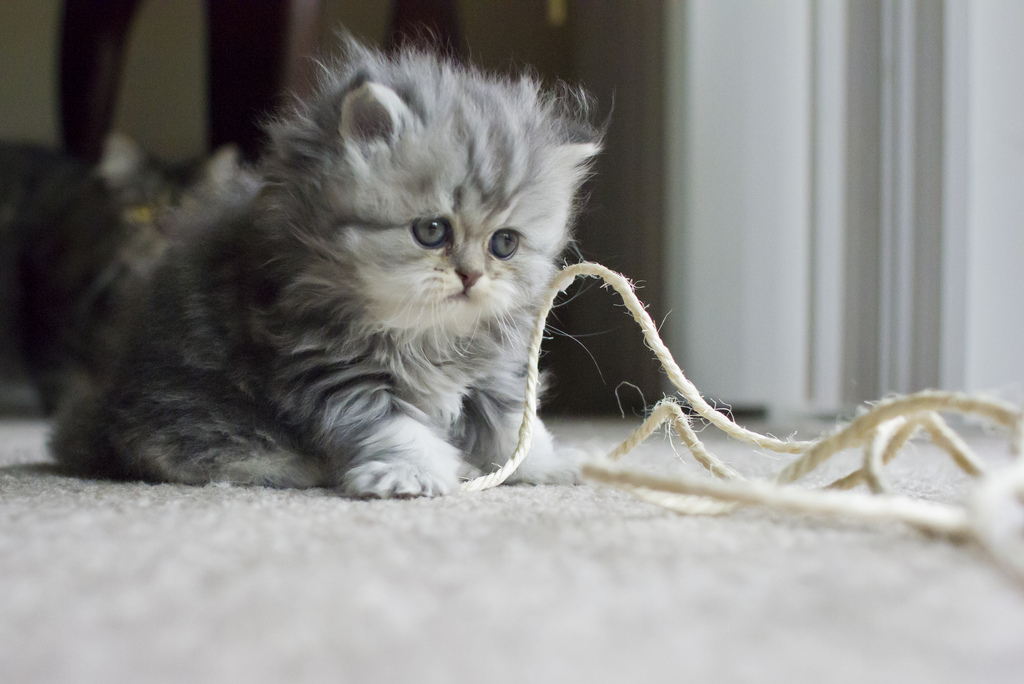
\includegraphics[width=0.5\textwidth]{images/kitten_string_flickr_albaraa.jpg} \\[-1.0em]
 %\small{Possibilities} \\[1.0em]
 %LT1 \\[1.0em]
 }
\author{\href{http://jon.dehdari.org}{Jon Dehdari}}
\frame{\titlepage}

\begin{frame}{Good Morning!}
	\begin{center}
	%\includegraphics[width=0.8\textwidth]{images/.jpg}
	\end{center}
\end{frame}

% what dense word vectors are, pix
\begin{frame}{Words as Integers}
\begin{itemize}
	\item Our previous representations of words (and word classes) have been fairly flat
	\item For example, the word `\textit{monkey}' can be represented as an integer, such as `7'
	\pause
	\item \textbf{One-hot encoding} represents that as: \\[0.4em]
		\begin{tabular}{|c|c|c|c|c|c|c|c|c|c|c|c|}
		    \hline
			%\colorbox{black}{\color{white}1}
			0 & 0 & 0 & 0 & 0 & 0 & 1 & 0 & 0 & 0 & \ldots & 0 \\
		    \hline
		\end{tabular}
	\pause

	\item and the word class containing `\textit{monkey}': \\[0.4em]
		\begin{tabular}{|c|c|c|c|}
		    \hline
			0 & 1 & 0 & 0 \\
		    \hline
		\end{tabular}

	\pause
	\item Both of these are sparse vectors of booleans, with just one entry having a `true' value
	\pause
	\item Either way, we're working with integers {\small (\ldots, -2, -1, 0, 1, 2, \ldots)}
\end{itemize}
\end{frame}


\begin{frame}{
\includegraphics[width=0.06\textheight]{images/real_madrid_cf.png} \hspace{1.5em} Words as $\mathbb{R}$eal Numbers}
\begin{itemize}
	\item We can do more with real numbers (eg. -1.5, 0.23, 55.01)
	\pause
	\item We can represent the word `\textit{monkey}' as a dense vector of real numbers: \\[0.4em]
		\begin{tabular}{|c|c|c|c|}
		    \hline
			0.38 & -1.27 & -0.55 & 1.44 \\
		    \hline
		\end{tabular}
	\pause
	\item We can have the plural form, `\textit{monkeys}' be close in that vector space: \\[0.4em]
		\begin{tabular}{|c|c|c|c|}
		    \hline
			\bf 0.35 & -1.27 & \bf -0.51 & 1.44 \\
		    \hline
		\end{tabular}
	\pause
	\item We can also have a related word, like `\textit{ape}' be close in that vector space, \emph{but in different directions}: \\[0.4em]
		\begin{tabular}{|c|c|c|c|}
		    \hline
			0.38 & \bf -1.33 & -0.55 & \bf 1.49 \\
		    \hline
		\end{tabular}
\end{itemize}
\end{frame}


% applications: analogy, qa, nnlm's
\begin{frame}{}
\begin{itemize}
	\item 
	\item 
\end{itemize}
\end{frame}


\begin{frame}{}
\begin{itemize}
	\item 
	\item 
\end{itemize}
\end{frame}


% models, relationship with projection layers of nnlm's
\begin{frame}{}
\begin{itemize}
	\item 
	\item 
\end{itemize}
\end{frame}


\begin{frame}{}
\begin{itemize}
	\item 
	\item 
\end{itemize}
\end{frame}


% word2vec: cbow, sg
\begin{frame}{}
\begin{itemize}
	\item 
	\item 
\end{itemize}
\end{frame}


\begin{frame}{}
\begin{itemize}
	\item 
	\item 
\end{itemize}
\end{frame}


% metaparameters: models, window size, normalization (softmax, neg. sampling)
\begin{frame}{}
\begin{itemize}
	\item 
	\item 
\end{itemize}
\end{frame}


\begin{frame}{}
\begin{itemize}
	\item 
	\item 
\end{itemize}
\end{frame}


% glove, maybe SVD-based approaches
\begin{frame}{}
\begin{itemize}
	\item 
	\item 
\end{itemize}
\end{frame}


\begin{frame}{}
\begin{itemize}
	\item 
	\item 
\end{itemize}
\end{frame}


% bilingual word vectors

\begin{frame}{}
\begin{itemize}
	\item 
	\item 
\end{itemize}
\end{frame}

\begin{frame}{}
\begin{itemize}
	\item 
	\item 
\end{itemize}
\end{frame}






% \begin{frame}{}
% \begin{block}{}
% \begin{itemize}
% 	\item 
% 	\item 
% 	\item 
% \end{itemize}
% \end{block}
% \end{frame}


\end{document}
